%\VignetteIndexEntry{The qsmooth user's guide}
%\VignettePackage{qsmooth}
%\VignetteEngine{knitr::knitr}
\documentclass{article}\usepackage[]{graphicx}\usepackage[usenames,dvipsnames]{color}
%% maxwidth is the original width if it is less than linewidth
%% otherwise use linewidth (to make sure the graphics do not exceed the margin)
\makeatletter
\def\maxwidth{ %
  \ifdim\Gin@nat@width>\linewidth
    \linewidth
  \else
    \Gin@nat@width
  \fi
}
\makeatother

\definecolor{fgcolor}{rgb}{0.345, 0.345, 0.345}
\newcommand{\hlnum}[1]{\textcolor[rgb]{0.686,0.059,0.569}{#1}}%
\newcommand{\hlstr}[1]{\textcolor[rgb]{0.192,0.494,0.8}{#1}}%
\newcommand{\hlcom}[1]{\textcolor[rgb]{0.678,0.584,0.686}{\textit{#1}}}%
\newcommand{\hlopt}[1]{\textcolor[rgb]{0,0,0}{#1}}%
\newcommand{\hlstd}[1]{\textcolor[rgb]{0.345,0.345,0.345}{#1}}%
\newcommand{\hlkwa}[1]{\textcolor[rgb]{0.161,0.373,0.58}{\textbf{#1}}}%
\newcommand{\hlkwb}[1]{\textcolor[rgb]{0.69,0.353,0.396}{#1}}%
\newcommand{\hlkwc}[1]{\textcolor[rgb]{0.333,0.667,0.333}{#1}}%
\newcommand{\hlkwd}[1]{\textcolor[rgb]{0.737,0.353,0.396}{\textbf{#1}}}%

\usepackage{framed}
\makeatletter
\newenvironment{kframe}{%
 \def\at@end@of@kframe{}%
 \ifinner\ifhmode%
  \def\at@end@of@kframe{\end{minipage}}%
  \begin{minipage}{\columnwidth}%
 \fi\fi%
 \def\FrameCommand##1{\hskip\@totalleftmargin \hskip-\fboxsep
 \colorbox{shadecolor}{##1}\hskip-\fboxsep
     % There is no \\@totalrightmargin, so:
     \hskip-\linewidth \hskip-\@totalleftmargin \hskip\columnwidth}%
 \MakeFramed {\advance\hsize-\width
   \@totalleftmargin\z@ \linewidth\hsize
   \@setminipage}}%
 {\par\unskip\endMakeFramed%
 \at@end@of@kframe}
\makeatother

\definecolor{shadecolor}{rgb}{.97, .97, .97}
\definecolor{messagecolor}{rgb}{0, 0, 0}
\definecolor{warningcolor}{rgb}{1, 0, 1}
\definecolor{errorcolor}{rgb}{1, 0, 0}
\newenvironment{knitrout}{}{} % an empty environment to be redefined in TeX

\usepackage{alltt}

\RequirePackage{/Library/Frameworks/R.framework/Versions/3.2/Resources/library/BiocStyle/resources/tex/Bioconductor}

\AtBeginDocument{\bibliographystyle{/Library/Frameworks/R.framework/Versions/3.2/Resources/library/BiocStyle/resources/tex/unsrturl}}


\setlength{\parskip}{1\baselineskip}
\setlength{\parindent}{0pt}

\title{The \texttt{qsmooth} user's guide}
\author{Kwame Okrah \texttt{okrah.kwame@gene.com} \and
Stephanie C. Hicks \texttt{shicks@jimmy.harvard.edu} \and
Hector Corrado Bravo \texttt{hcorrada@gmail.com} \and
Rafael A. Irizarry \texttt{rafa@jimmy.harvard.edu} }

\date{Modified: March 5, 2015.  Compiled: \today}
\IfFileExists{upquote.sty}{\usepackage{upquote}}{}
\begin{document}

\maketitle
 
\tableofcontents

\section{Introduction}

In the analysis of high-throughput gene expression data, 
normalization strategies based solely on observed data 
without any external information often make the following assumption: 
for each sample in the study only a minority of genes are expected to be 
differentially epxressed or that an equivalent number of genes increase 
and decrease across the different biological conditions 
\cite{aanes2014normalization}.

This assumption can be interpreted in different ways 
leading to different normalization procedures.
For example, in one normalization procedure, the method assumes 
the mean expression level across genes should be the same across samples 
\cite{robinson2010scaling}. In contrast, 
quantile normalization assumes the statistical distribution of gene expression 
is the same across all samples \cite{bolstad2003comparison}. 
Other normalization methods based on {\it housekeeping genes} assume genes 
play a critical role in basic cellular pathways and as such should be 
expressed all the time at an equal rate independent of samples
\cite{eisenberg2013human}.
While these assumptions may be reasonable in certain experiments, 
they may not always be appropriate \cite{loven2012revisiting, hicks}.
For example, mRNA content has been shown to fluctuate significantly 
during zebrafish early developmental stages \cite{aanes2014normalization}.
Similarily, cells expressing high levels of c-Myc undergo 
transcriptional amplification causing a 2 to 3 fold change in global 
gene expression compared to cells expressiong low c-Myc 
\cite{loven2012revisiting}. In these cases with global changes of 
gene expression between biological conditions such as in cancer, 
transcriptional amplification or early developmental stages of zebrafish, 
quantile normalization is not an appropriate normalization method. In 
these cases, we can consider a more relaxed assumption about the data, namely
that the statistical distribution of each sample should be the same 
within biological conditions or groups (compared to the more stringent 
assumption of quantile normalization, which states the statistical 
distribution is the same across all samples).

In this vignette we introduce a generalization of quantile normalization, 
referred to as \textbf{smooth quantile normalization} (\texttt{\bf{qsmooth}}), 
which is a weighted average of the two types of assumptions about the data. 
The \texttt{qsmooth} R-package contains the \texttt{qsmooth()} function, 
which computes a weight at every quantile that compares the variability between
groups relative to within groups. In one extreme quantile normalization is applied
and in the other extreme quantile normalization within each biological condition
is applied. The weight shrinks the group-level quantile normalized data
towards the overall reference quantiles if variability between groups is sufficiently smaller than
the variability within groups. 
The algorithm is described in Figure \ref{algo} below. 

Let \texttt{gene(g)} denote the ${g}^{th}$ row after sorting each column in the data. 
For each row, \texttt{gene(g)}, we compute the weight $w_{(g)} \in [0, 1]$, 
where a weight of 0 implies quantile normalization within groups is applied and
a weight of 1 indicates quantile normalization is applied.
The weight at each row depends on the between group sum of squares
$\hbox{SSB}_{(g)}$ and total sum of squares $\hbox{SST}_{(g)}$, 
as follows:
\begin{equation}
w_{(g)} = \hbox{median} \{1 - \hbox{SSB}_{(i)} / \hbox{SST}_{(i)} | ~i = g-k, \dots, g, \dots, g+k \},
\end{equation}
where $k=$ floor(Total number of genes * 0.05). The number 0.05 is a flexible 
parameter that can be altered to change the window of the number of genes 
considered. In this way, we can use a rolling median to borrow information 
from neighboring genes in the weight.

\begin{figure}[!h]
\begin{center}
\includegraphics[width=\columnwidth]{qsmooth_algo.pdf}
\end{center}
\small\normalsize
\caption[qsmooth algorithm]
         {{\bf The qsmooth algorithm}}
\label{algo}
\end{figure}


%--------------- Getting Started
\section{Getting Started}

Load the package in R
\begin{knitrout}
\definecolor{shadecolor}{rgb}{0.969, 0.969, 0.969}\color{fgcolor}\begin{kframe}
\begin{alltt}
\hlkwd{library}\hlstd{(qsmooth)}
\end{alltt}
\end{kframe}
\end{knitrout}



%--------------- Rat bodymap
\section{Data} 

The \texttt{\bf{bodymapRat}} package contains an \texttt{ExpressionSet} 
of 652 RNA-Seq samples from a comprehensive rat transcriptomic BodyMap study. 
This data was derived from the raw FASTQ files obtained from Yu et al. (2013) 
\cite{Yu:2014}. It contains expression levels from 11 organs in male and female rats
at 4 developmental stages. We will use a subset of this data in this vignette.

The R-package bodymapRat can be installed from GitHub 
(\texttt{https://github.com/stephaniehicks/bodymapRat}) using the R package 
\texttt{\bf{devtools}}.

\begin{knitrout}
\definecolor{shadecolor}{rgb}{0.969, 0.969, 0.969}\color{fgcolor}\begin{kframe}
\begin{alltt}
\hlkwd{library}\hlstd{(devtools)}
\hlkwd{install_github}\hlstd{(}\hlstr{"stephaniehicks/bodymapRat"}\hlstd{)}
\end{alltt}
\end{kframe}
\end{knitrout}


\subsection{bodymapRat example 1}

The first example is based a dataset
which contains lung samples from 21 week old male and female rats. 
Four samples are from males and four samples are from females.

\begin{knitrout}
\definecolor{shadecolor}{rgb}{0.969, 0.969, 0.969}\color{fgcolor}\begin{kframe}
\begin{alltt}
\hlkwd{library}\hlstd{(Biobase)}
\hlkwd{library}\hlstd{(bodymapRat)}

\hlstd{pd} \hlkwb{=} \hlkwd{pData}\hlstd{(bodymapRat)} \hlcom{# grab pheno data}

\hlcom{# Subset samples from bodymapRat}
\hlstd{sel} \hlkwb{=} \hlstd{pd}\hlopt{$}\hlstd{organ} \hlopt \hlstr{"Lung"} \hlcom{# select lung samples}
\hlstd{sel} \hlkwb{=} \hlstd{sel} \hlopt{&} \hlstd{pd}\hlopt{$}\hlstd{stage} \hlopt{==} \hlnum{21} \hlcom{# select stage 21 weeks}
\hlstd{sel} \hlkwb{=} \hlstd{sel} \hlopt{&} \hlstd{pd}\hlopt{$}\hlstd{techRep} \hlopt{==} \hlnum{1} \hlcom{# select biological replicates }

\hlcom{# Filter out low count genes}
\hlstd{keep} \hlkwb{=} \hlkwd{rowMeans}\hlstd{(}\hlkwd{exprs}\hlstd{(bodymapRat))} \hlopt{>} \hlnum{10}
\hlstd{data1} \hlkwb{=} \hlstd{bodymapRat[keep, sel]}
\end{alltt}
\end{kframe}
\end{knitrout}

Below are the boxplots and the density plots of the data after after adding 1 
and transforming the raw counts on the \texttt{log2()} scale 
(i.e. \texttt{log2(counts+1)}).

\begin{knitrout}
\definecolor{shadecolor}{rgb}{0.969, 0.969, 0.969}\color{fgcolor}

{\centering 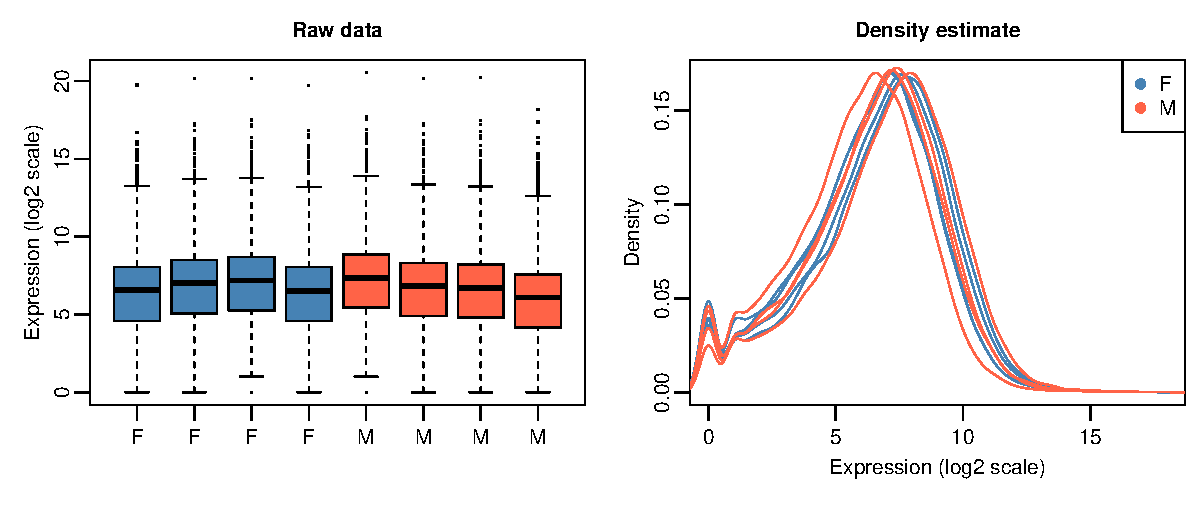
\includegraphics[width=\maxwidth]{figure/raw1-1} 

}



\end{knitrout}

To run the \texttt{qsmooth()} algorithm on the log transformed raw counts, 
we must specify the group-level information for each sample. In this example 
we will use gender as the group-level factor. 

\begin{knitrout}
\definecolor{shadecolor}{rgb}{0.969, 0.969, 0.969}\color{fgcolor}\begin{kframe}
\begin{alltt}
\hlstd{norm.data1} \hlkwb{=} \hlkwd{qsmooth}\hlstd{(}\hlkwc{exprs}\hlstd{=data1,} \hlkwc{groups}\hlstd{=sex,} \hlkwc{plot}\hlstd{=}\hlnum{TRUE}\hlstd{)}
\end{alltt}
\end{kframe}

{\centering 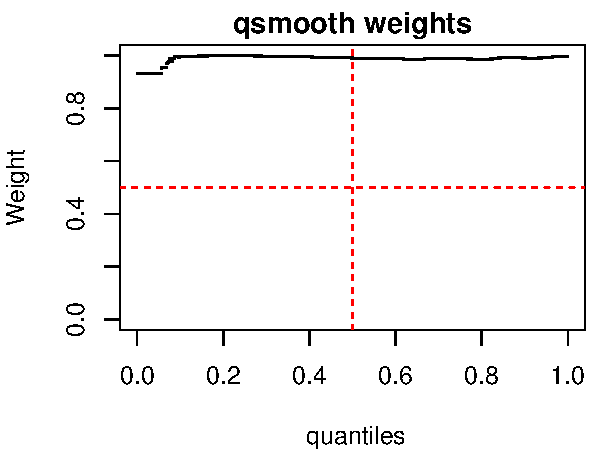
\includegraphics[width=\maxwidth]{figure/qsmooth1-1} 

}



\end{knitrout}

The parameter \texttt{plot=TRUE} indicates that we want to see the weight 
of interpolation. Weights are computed for each quantile in the data set.
A weight of 1 indicates quantile normalization is applied,
where as a weight of 0 indicates quantile normalization
within the groups is applied. See Figure \ref{algo} for more details on 
the weights.

In this example, the weights are close to 1 across all the quantiles 
indicating that there is no major difference between the group-level quantiles 
in the female and male rats. Here, the \texttt{qsmooth()} algorithm returns a 
normalized data set that is nearly identical (for practical purposes)
to the conventional quantile normalization. 

Below are the boxplots and density plots after applying the \texttt{qsmooth()} 
normalization.
\begin{knitrout}
\definecolor{shadecolor}{rgb}{0.969, 0.969, 0.969}\color{fgcolor}

{\centering 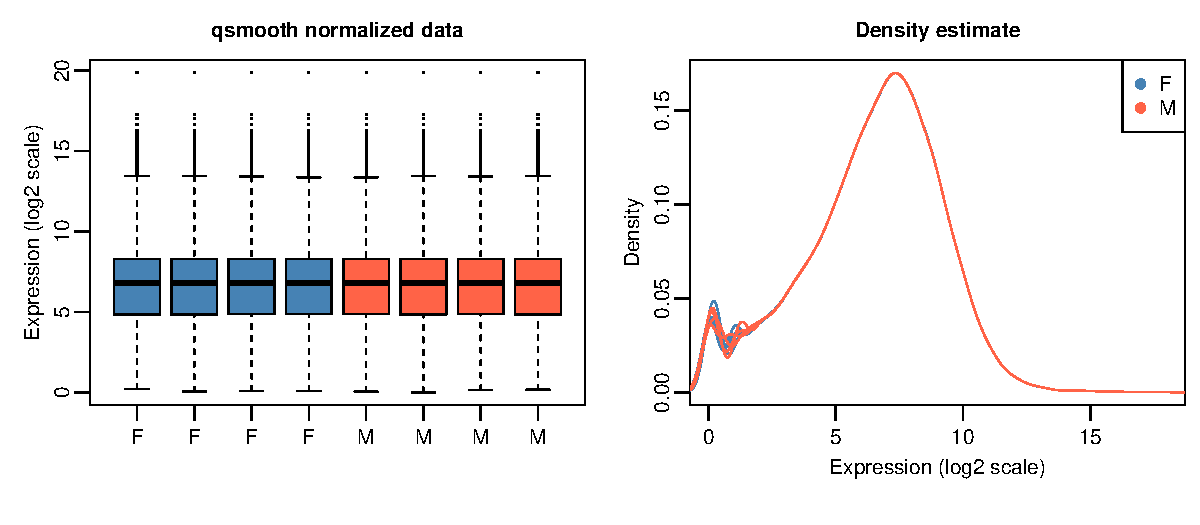
\includegraphics[width=\maxwidth]{figure/norm_data1-1} 

}



\end{knitrout}

\subsection{bodymapRat example 2}

The second example is based a dataset containing lung and liver samples from 
21 week old male and female rats. Eight samples are males and eight 
samples are females.



Below are the boxplots and the density plots of the raw data after after adding 1 
and transforming the raw counts on the \texttt{log2()} scale 
(i.e. \texttt{log2(counts+1)}).

\begin{knitrout}
\definecolor{shadecolor}{rgb}{0.969, 0.969, 0.969}\color{fgcolor}

{\centering 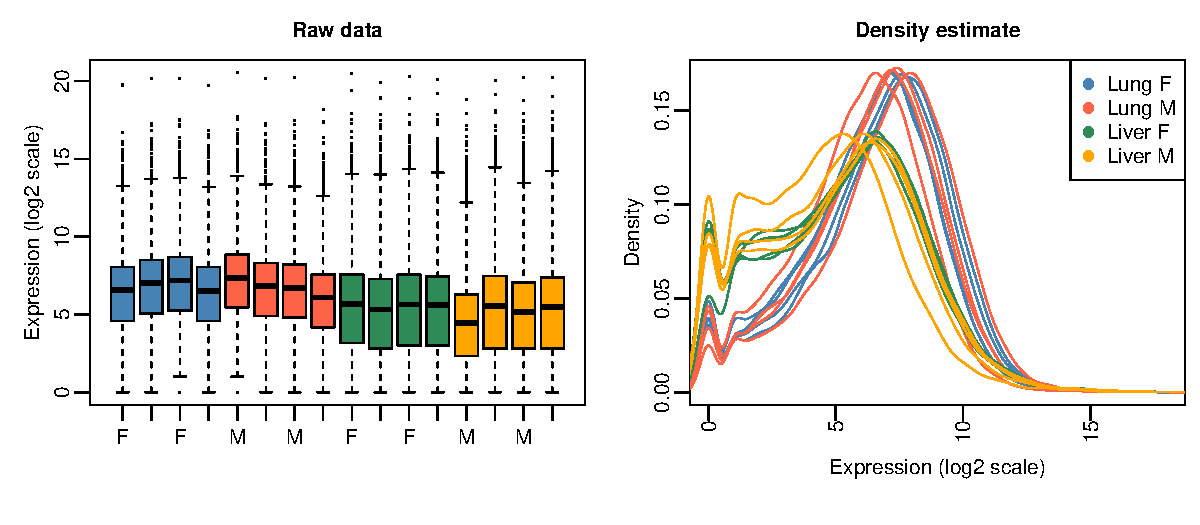
\includegraphics[width=\maxwidth]{figure/norm_data2-1} 

}



\end{knitrout}

To run the \texttt{qsmooth()} algorithm on the log transformed raw counts, 
we must specify the group-level information for each sample. In this example 
we will use gender and organ as the group-level factor. 

\begin{knitrout}
\definecolor{shadecolor}{rgb}{0.969, 0.969, 0.969}\color{fgcolor}\begin{kframe}
\begin{alltt}
\hlstd{norm.data2} \hlkwb{=} \hlkwd{qsmooth}\hlstd{(}\hlkwc{exprs}\hlstd{=data2,} \hlkwc{groups}\hlstd{=}\hlkwd{paste0}\hlstd{(sex, organ),} \hlkwc{plot}\hlstd{=}\hlnum{TRUE}\hlstd{)}
\end{alltt}
\end{kframe}

{\centering 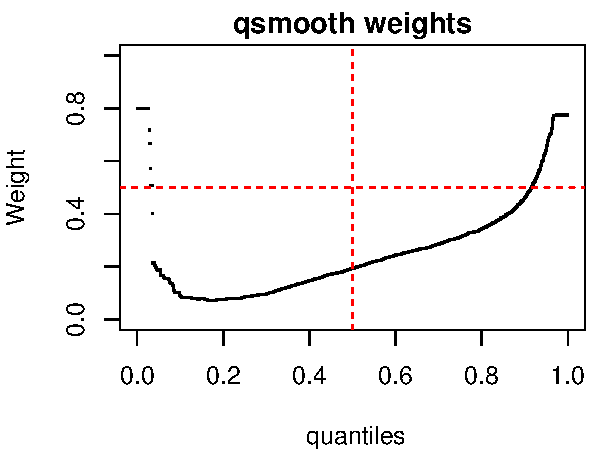
\includegraphics[width=\maxwidth]{figure/qsmooth12-1} 

}



\end{knitrout}

In this example, the weights are mostly below 0.2 before the median quantile
(0.5) and increase steadily to 0.8. This indicates there is a difference 
in the statistical distributions of the samples between the groups. 
In this case, the conventional quantile normalization is not appropriate. 

Below are the boxplots and density plots after applying the \texttt{qsmooth()} 
normalization. Note: within the liver samples males and females show a 
small difference that is not in the lung samples.

\begin{knitrout}
\definecolor{shadecolor}{rgb}{0.969, 0.969, 0.969}\color{fgcolor}

{\centering 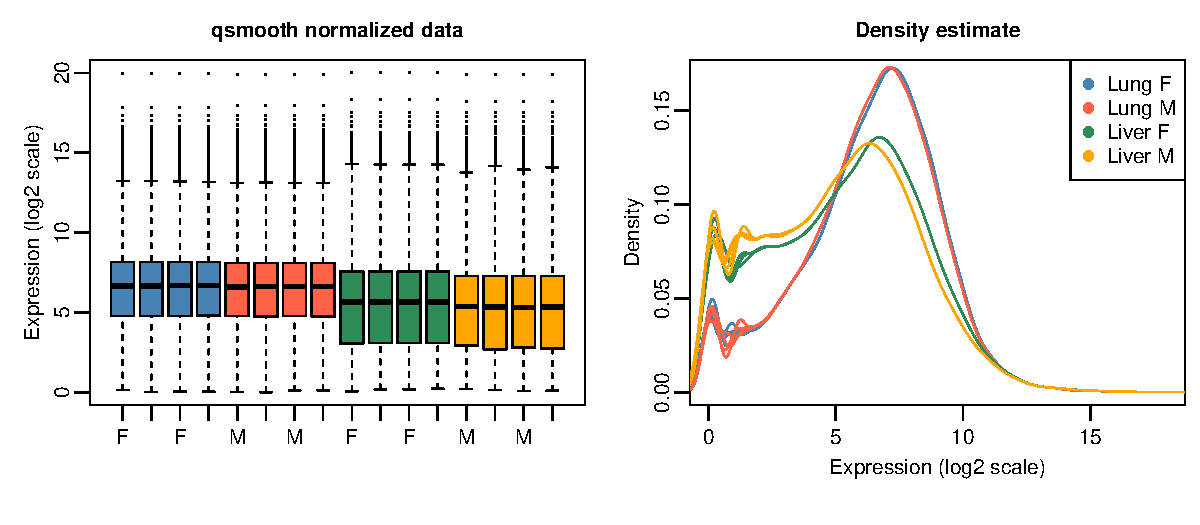
\includegraphics[width=\maxwidth]{figure/norm_data12-1} 

}



\end{knitrout}

%------------ qsmooth fucntion
\section{Additional information for the \texttt{qsmooth()} function}
The \texttt{qsmooth()} function accepts five parameters.
\begin{enumerate}
\item \texttt{exprs}: for counts use \texttt{log2(raw counts + 1))}, 
for microarray use \texttt{log2(raw intensities)}
\item \texttt{groups}: groups to which samples belong (character vector)
\item \texttt{norm.factors}: scaling normalization factors ({\bf optional})
\item \texttt{plot}: plot weights? (\texttt{default=FALSE}) ({\bf optional})
\item \texttt{plot}: window window size for running median 
(defined as a fraction of the number of rows of exprs) (\texttt{default=0.05})
\end{enumerate}
The \texttt{qsmooth} function requires an expression matrix and a 
character vector or factor specifying the group-level information for that 
sample. The \texttt{plot} parameter is optional. It specifies whether or
not the weights should be plotted. It is set to \texttt{FALSE} as default. 
The \texttt{norm.factors} allows the user to specify a 
vector of scaling factors that will be used to modify the 
expression data set prior to applying the qsmooth algorithm 
(see discussion on spike-in below).


\subsection{External RNA Control Consortium Spike-in Mixes}

The External RNA Control Consortium (ERCC)
is a collaborative group of academic, private, and 
public organizations hosted at the 
National Institutes of Standard and Technology (NIST)
\cite{baker2005external, external2005proposed}. 
The ERCC has developed a set of 92 mRNA controls 
(20-mer poly(A) tails) that can be used in gene expression 
platforms such as RNA-seq, DNA microarrays, and 
quantitative real-time reverse transcriptase PCR (qRT-PCR).
The 92 mRNA transcripts are divided into 4 groups labelled
A, B, C, and D.  
Each group contains 23 mRNA transcripts 
spanning a $10^6$-fold concentration range.
There are two ERCC control spike-in mixes: mix 1 and mix 2. 
The molar concentration ratios of mix 1 to mix 2 are 4, 1, 0.67, and 
0.5 for group A, B, C, and D respectively. 
When the ERCC spike-in mix is used as a 
control in the experiment its measurements can be used 
as part of the data normalization process
\cite{loven2012revisiting, risso2014normalization}.

In Figure \ref{ercc} we show the distribution of the 
{\bf true and known} concentration of each of the 92 "genes" in 
mix 1 and mix 2. Based on these plots we can make the 
assumption that the mix 1 and mix 2 "transcriptomes" have
the same distribution 
(even though certain "genes" are differentially expressed).

\begin{figure}[!h]
\begin{center}
\includegraphics[width=\columnwidth]{ercc.pdf}
\end{center}
\small\normalsize
\caption[qsmooth algorithm]
         {{\bf ERCC spike-in mix 1 and mix 2}}
\label{ercc}
\end{figure}

\subsection{Pre-specified scaling factors}
This is an example of incorporating the ERCC spike-ins into \texttt{qsmooth()}
as pre-specified scaling factors. 

\begin{knitrout}
\definecolor{shadecolor}{rgb}{0.969, 0.969, 0.969}\color{fgcolor}\begin{kframe}
\begin{alltt}
\hlstd{ercc} \hlkwb{=} \hlstd{data2[}\hlkwd{grep}\hlstd{(}\hlstr{"^ERCC"}\hlstd{,} \hlkwd{rownames}\hlstd{(data2)), ]}
\hlkwd{dim}\hlstd{(ercc)}
\end{alltt}
\begin{verbatim}
## [1] 48 16
\end{verbatim}
\begin{alltt}
\hlstd{errcSF} \hlkwb{=} \hlkwd{apply}\hlstd{(ercc,} \hlnum{2}\hlstd{, median)}
\hlstd{norm.data3} \hlkwb{=} \hlkwd{qsmooth}\hlstd{(}\hlkwc{exprs}\hlstd{=}\hlkwd{t}\hlstd{(}\hlkwd{t}\hlstd{(data2)}\hlopt{/}\hlstd{errcSF),} \hlkwc{groups}\hlstd{=}\hlkwd{paste0}\hlstd{(sex, organ),} \hlkwc{plot}\hlstd{=}\hlnum{TRUE}\hlstd{)}
\end{alltt}
\end{kframe}

{\centering 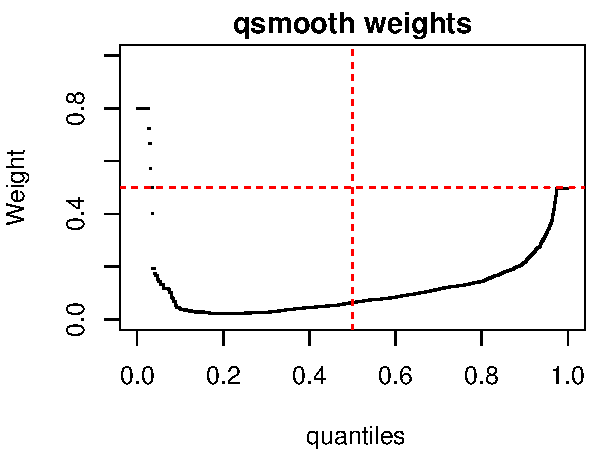
\includegraphics[width=\maxwidth]{figure/qsmooth14-1} 

}



\end{knitrout}

\begin{knitrout}
\definecolor{shadecolor}{rgb}{0.969, 0.969, 0.969}\color{fgcolor}

{\centering 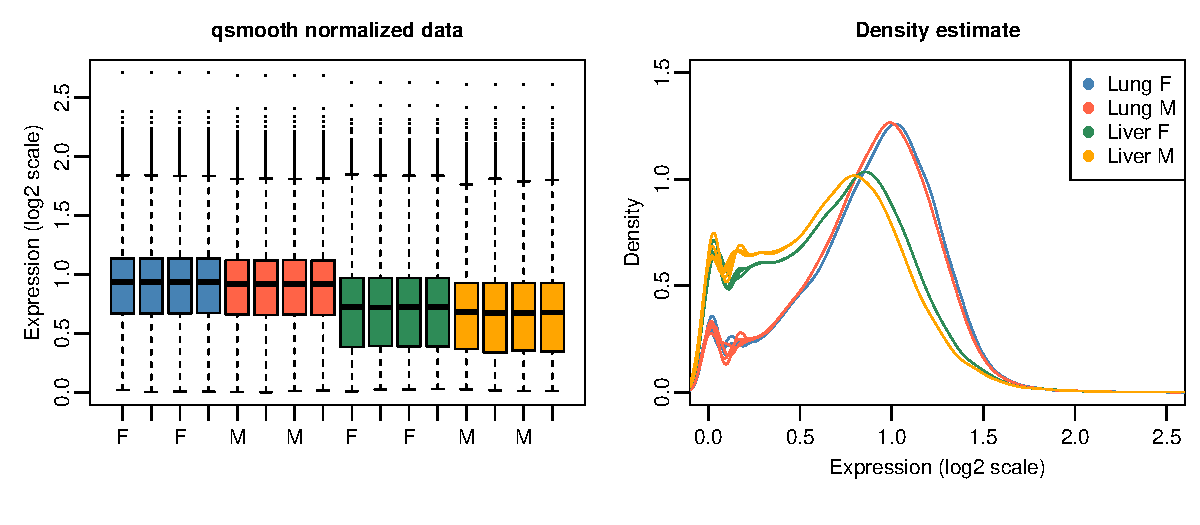
\includegraphics[width=\maxwidth]{figure/norm_data14-1} 

}



\end{knitrout}

\section{SessionInfo}

\begin{knitrout}
\definecolor{shadecolor}{rgb}{0.969, 0.969, 0.969}\color{fgcolor}\begin{kframe}
\begin{alltt}
\hlkwd{sessionInfo}\hlstd{()}
\end{alltt}
\begin{verbatim}
## R version 3.2.2 (2015-08-14)
## Platform: x86_64-apple-darwin13.4.0 (64-bit)
## Running under: OS X 10.11.1 (El Capitan)
## 
## locale:
## [1] en_US.UTF-8/en_US.UTF-8/en_US.UTF-8/C/en_US.UTF-8/en_US.UTF-8
## 
## attached base packages:
## [1] parallel  stats     graphics  grDevices datasets  utils     methods   base     
## 
## other attached packages:
## [1] bodymapRat_0.0.1    Biobase_2.30.0      BiocGenerics_0.16.1 qsmooth_0.0.0.9000 
## [5] knitr_1.11         
## 
## loaded via a namespace (and not attached):
## [1] BiocStyle_1.8.0 magrittr_1.5    formatR_1.2.1   tools_3.2.2     stringi_1.0-1  
## [6] highr_0.5.1     stringr_1.0.0   evaluate_0.8
\end{verbatim}
\end{kframe}
\end{knitrout}

\bibliography{myrefs}

\end{document}
